\documentclass[10pt,pdf,hyperref={unicode}]{beamer}

\usepackage{lmodern}

\usepackage[T2A]{fontenc}
\usepackage[utf8]{inputenc}

%\usepackage{tikz}
%\usepackage{tikz-qtree}

\setbeamertemplate{navigation symbols}{}

\usetheme{CambridgeUS}

\usecolortheme{seahorse}

\title[IntelliJ Rust Intentions pack]{IntelliJ Rust \\ Intentions pack}   
\institute[]{ Computer Science Center \\
	Руководитель: Алексей Кладов
}
\author{Владимир Харитонов} 

\date{\today} 

\begin{document}
\begin{frame}
\titlepage
\end{frame} 

\begin{frame}
\frametitle{Язык Rust} 
	Разрабатывается с 2009 года компанией Mozilla.
%	\begin{block}{Особенности языка}
%	\begin{itemize}
%		\item Мультипарадигменность 
%		\item Система типов
%		\item Система владения и проверки заимствований
%	\end{itemize}
%	\end{block}

    \begin{block}{Особенности}
        \begin{itemize}
            \item Абстракция без накладных расходов 
            \item Безопасность памяти без GC (RAII + lifetimes)
            \item Отсутствие гонок данных при конкурентном программировании
        \end{itemize}
    \end{block}
    \vfill
    {
        \centering
	    
\includegraphics[scale = 0.2]{rust-logo-512x512-blk.png} \\
    }
\end{frame}

\begin{frame}
	\frametitle{IDE для Rust} 
	\begin{itemize}
		\item IntelliJ IDEA
		\item Eclipse
		\item Visual Studio
        \item Sublime
		\item Emacs
		\item Vim
		\item ...
	\end{itemize}
\end{frame}

\begin{frame}
	\frametitle{Постановка задачи} 
	Возможности плагина:
	\begin{itemize}
		\item Вывод типов
		\item Разрешение ссылок(go to definition)
		\item Автоформатирование
        \item Поддержка Cargo(система сборки и менеджер пакетов)
	\end{itemize}
	\vfill
	Пополнить плагин стандартными для IDEA "умными фичами":
	\begin{itemize}
		\item Postfix templates
		\item Surround with...
		\item Intentions
	\end{itemize}
\end{frame}

\begin{frame}
	\frametitle{Пример. Postfix tempalte "match"} 
	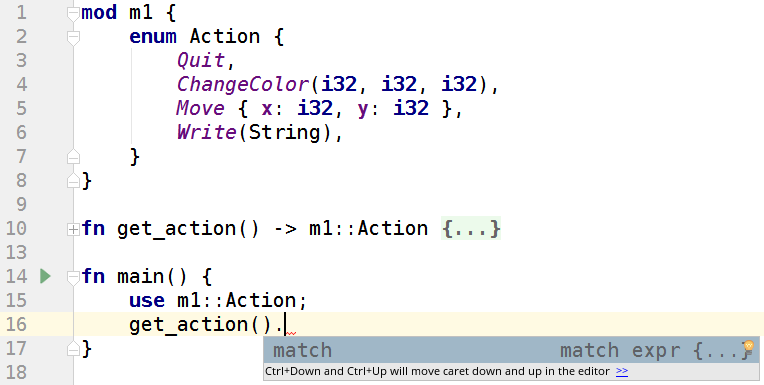
\includegraphics[scale = 0.6]{match_before.png}
\end{frame}

\begin{frame}
    \frametitle{Psi-дерево} 
	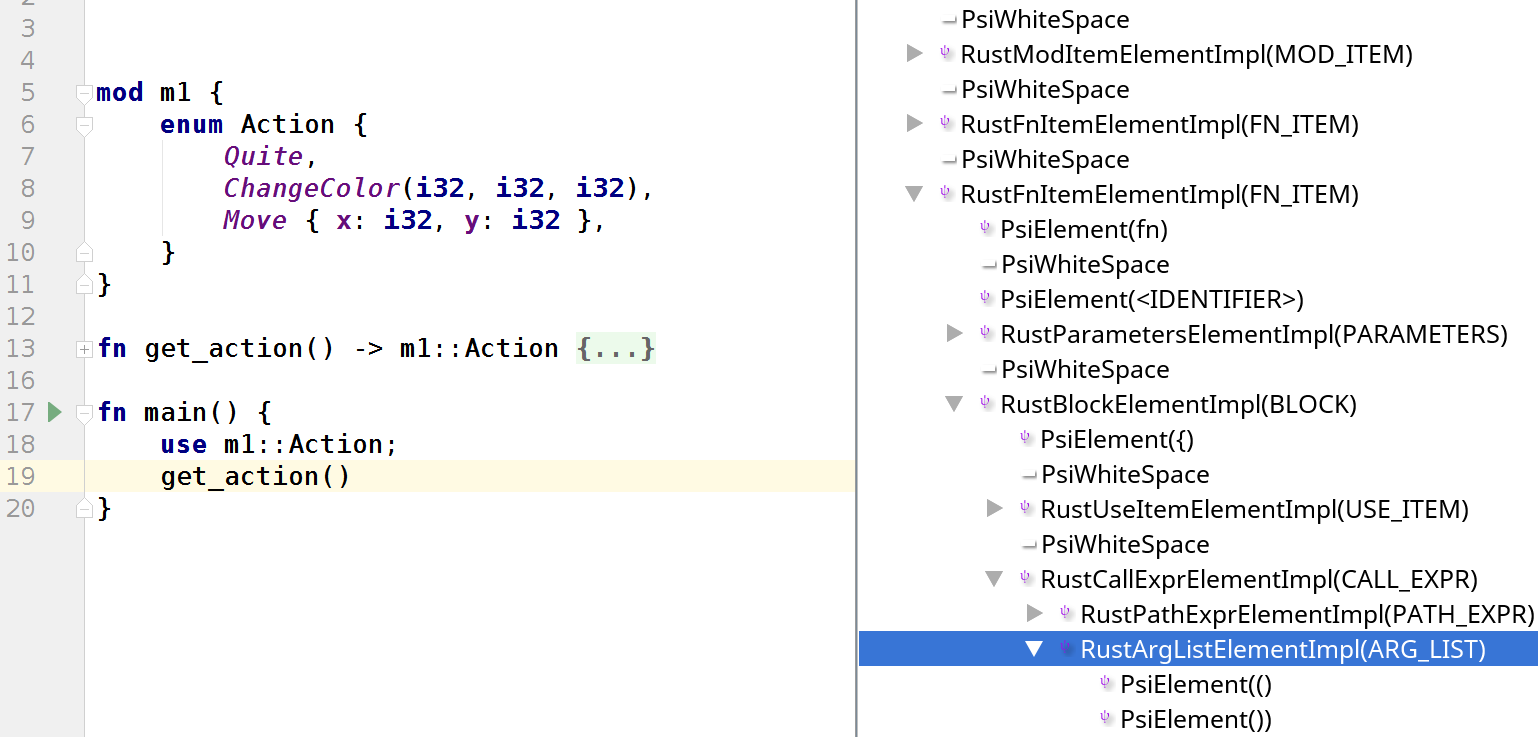
\includegraphics[scale = 0.3]{psi1.png}
\end{frame}

\begin{frame}
	\frametitle{Postfix tempalte "match". Результат} 
	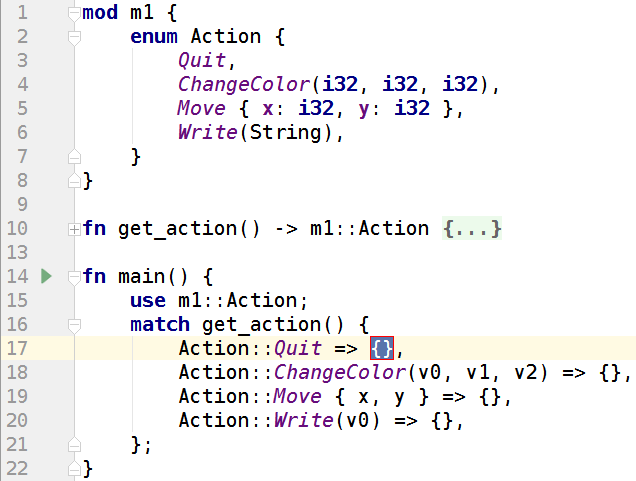
\includegraphics[scale = 0.6]{match_after.png}
\end{frame}

\begin{frame}
	\frametitle{Psi-дерево} 
	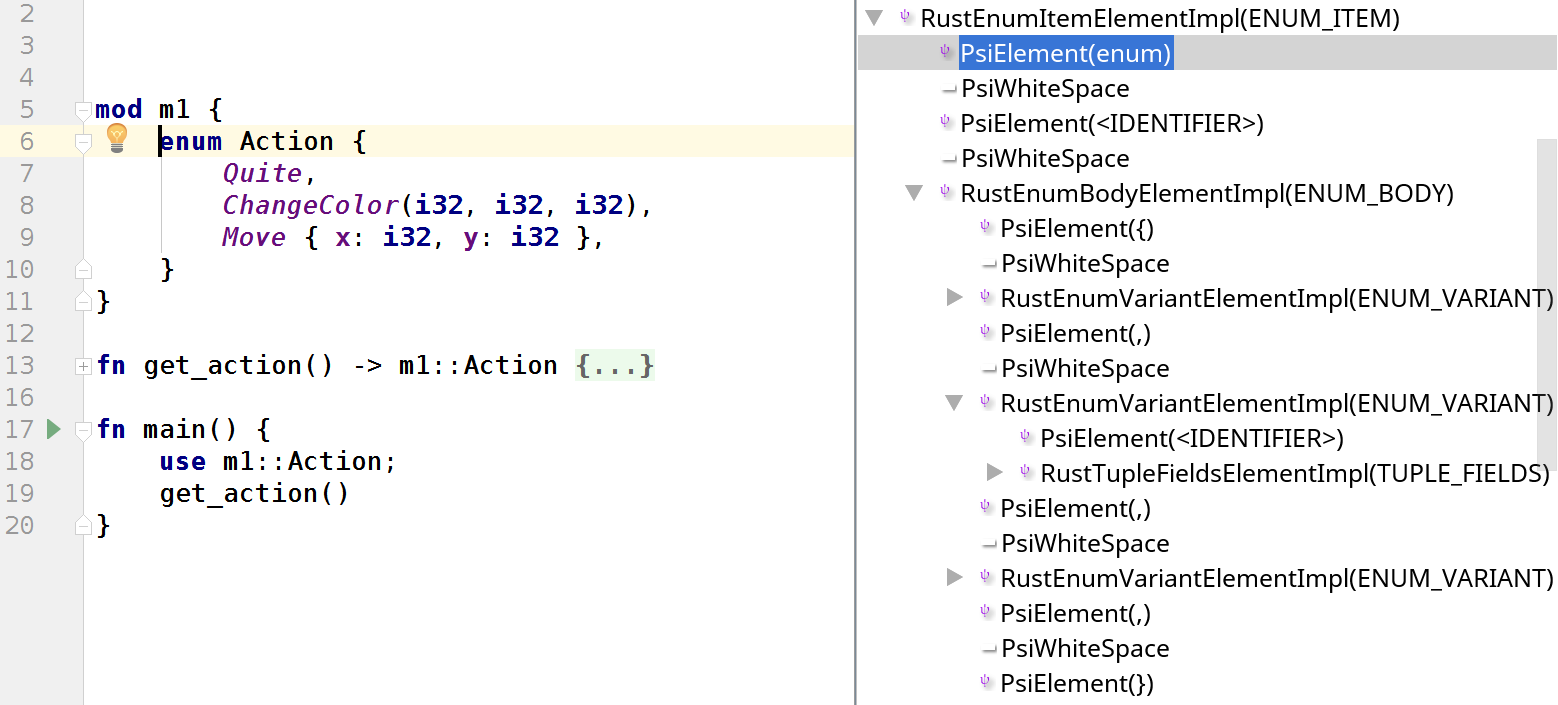
\includegraphics[scale = 0.3]{psi2.png}
\end{frame}


\begin{frame}
	\frametitle{Match to let if intentions} 
	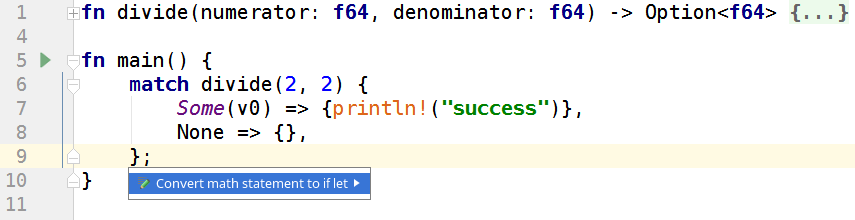
\includegraphics[scale = 0.5]{match2let_if_before.png}\\
	{
	\centering
	$\Downarrow$ \\
	}
	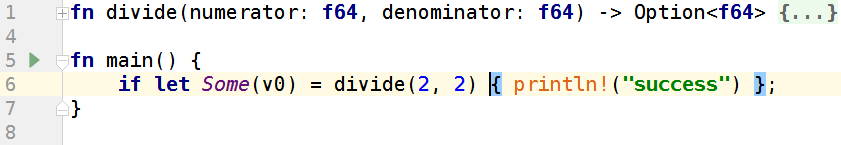
\includegraphics[scale = 0.5]{match2let_if_after.png}
\end{frame}

%\begin{frame}
%	\frametitle{Surround with loop} 
%	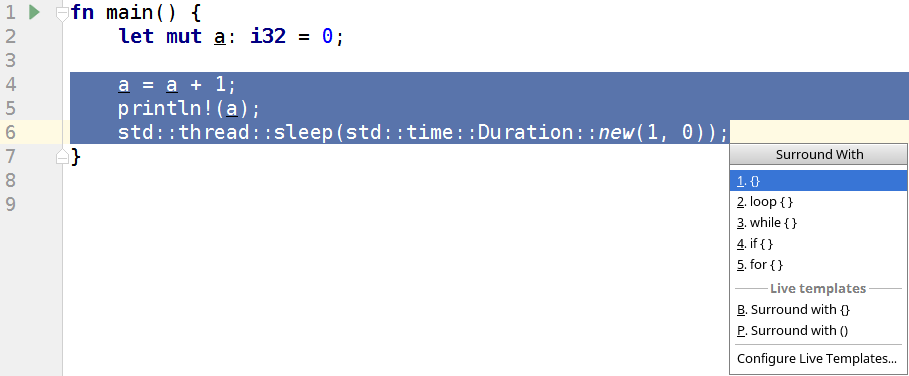
\includegraphics[scale = 0.5]{loop_before.png}\\
%	{
%		\centering $\Downarrow$ \\
%	}
%	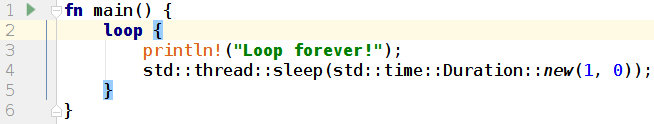
\includegraphics[scale = 0.5]{loop_after.png}
%\end{frame}

\begin{frame}
	\frametitle{Все фичи} 
	\begin{columns}
		\begin{column}{0.4\textwidth}
			\begin{block}{Postfix templates}
				\begin{itemize}
					\item if / else
					\item while / while not
					\item match
					\item paren 
					\item lambda
					\item assert, assert\_eq
					\item let, val, var
					\item for
				\end{itemize}
			\end{block}
			
			\begin{block}{Expression surround with}
				\begin{itemize}
					\item if, while
					\item скобки ()
					\item отрицание !
				\end{itemize}
			\end{block}
		\end{column}
		
		\begin{column}{0.4\textwidth}			
			\begin{block}{Statements surround with}
				\begin{itemize}
					\item if
					\item while
					\item loop
					\item for
					\item скобки {}
				\end{itemize}
			\end{block}
			
			\begin{block}{Intentions}			
				\begin{itemize}
					\item Добавление ветви else
					\item Добавление/удаление \{\}
					\item Match to let if
					\item Un-elide lifetimes
				\end{itemize}
			\end{block}	
		\end{column}
\end{columns}
\end{frame}

\begin{frame}
	\begin{block}{Технологии}
		\begin{itemize}
			\item Rust
			\item Idea plugin API
			\item Kotlin
			\item GitHub
		\end{itemize}
	\end{block}	
	
	\begin{block}{Plugin}
		\href
		{https://intellij-rust.github.io/}
		{https://intellij-rust.github.io/}
		\\
		\href
		{https://github.com/intellij-rust/intellij-rust.git}
		{https://github.com/intellij-rust/intellij-rust.git}
	\end{block}		
\end{frame}

\end{document}
